\documentclass[sigconf]{acmart}

%%
%% \BibTeX command to typeset BibTeX logo in the docs
\AtBeginDocument{%
  \providecommand\BibTeX{{%
    \normalfont B\kern-0.5em{\scshape i\kern-0.25em b}\kern-0.8em\TeX}}}

%% Rights management information.  This information is sent to you
%% when you complete the rights form.  These commands have SAMPLE
%% values in them; it is your responsibility as an author to replace
%% the commands and values with those provided to you when you
%% complete the rights form.
\setcopyright{acmcopyright}
\copyrightyear{2018}
\acmYear{2018}
\acmDOI{10.1145/1122445.1122456}

%% These commands are for a PROCEEDINGS abstract or paper.
\acmConference[FPGA'20]{International Symposium on Field-Programmable Gate Arrays}{February 23--25, 2020}{Monterey, CA, USA}
\acmYear{2020}
\acmBooktitle{FPGA '20: International Symposium on Field-Programmable Gate Arrays,
  February 23--25, 2020, Monterey, CA}
\acmPrice{15.00}
\acmISBN{978-1-4503-9999-9/18/06}


%%
%% Submission ID.
%% Use this when submitting an article to a sponsored event. You'll
%% receive a unique submission ID from the organizers
%% of the event, and this ID should be used as the parameter to this command.
%%\acmSubmissionID{123-A56-BU3}

%%
%% The majority of ACM publications use numbered citations and
%% references.  The command \citestyle{authoryear} switches to the
%% "author year" style.
%%
%% If you are preparing content for an event
%% sponsored by ACM SIGGRAPH, you must use the "author year" style of
%% citations and references.
%% Uncommenting
%% the next command will enable that style.
%%\citestyle{acmauthoryear}

%%
%% end of the preamble, start of the body of the document source.

%%%%%%%%%%%%%%%%%%%%%%%%%%%%%%%%%%%%%%%%%%%%%%%%%%%%%%%%%%%%%%%%%%%%%%%%%%%%%%%%%%
% Packages & Macros
%%%%%%%%%%%%%%%%%%%%%%%%%%%%%%%%%%%%%%%%%%%%%%%%%%%%%%%%%%%%%%%%%%%%%%%%%%%%%%%%%%
\usepackage{booktabs} % For formal tables

\usepackage{textcomp}
\usepackage{xcolor}
\usepackage{caption}


% *** GRAPHICS RELATED PACKAGES ***
%
%\usepackage[pdftex]{graphicx}

\usepackage[export]{adjustbox}
%\usepackage{color}


% *** MATH PACKAGES ***
%
\usepackage{amsmath,amssymb,amsfonts}
% A popular package from the American Mathematical Society that provides
% many useful and powerful commands for dealing with mathematics.
%
% Note that the amsmath package sets \interdisplaylinepenalty to 10000
% thus preventing page breaks from occurring within multiline equations. Use:
%\interdisplaylinepenalty=2500
% after loading amsmath to restore such page breaks as IEEEtran.cls normally
% does. amsmath.sty is already installed on most LaTeX systems. The latest
% version and documentation can be obtained at:
% http://www.ctan.org/pkg/amsmath




% *** ALIGNMENT PACKAGES ***
%
\usepackage{array}
% Frank Mittelbach's and David Carlisle's array.sty patches and improves
% the standard LaTeX2e array and tabular environments to provide better
% appearance and additional user controls. As the default LaTeX2e table
% generation code is lacking to the point of almost being broken with
% respect to the quality of the end results, all users are strongly
% advised to use an enhanced (at the very least that provided by array.sty)
% set of table tools. array.sty is already installed on most systems. The
% latest version and documentation can be obtained at:
% http://www.ctan.org/pkg/array


% *** FLOAT PACKAGES ***
%
\usepackage{fixltx2e}
% fixltx2e, the successor to the earlier fix2col.sty, was written by
% Frank Mittelbach and David Carlisle. This package corrects a few problems
% in the LaTeX2e kernel, the most notable of which is that in current
% LaTeX2e releases, the ordering of single and double column floats is not
% guaranteed to be preserved. Thus, an unpatched LaTeX2e can allow a
% single column figure to be placed prior to an earlier double column
% figure.
% Be aware that LaTeX2e kernels dated 2015 and later have fixltx2e.sty's
% corrections already built into the system in which case a warning will
% be issued if an attempt is made to load fixltx2e.sty as it is no longer
% needed.
% The latest version and documentation can be found at:
% http://www.ctan.org/pkg/fixltx2e



% *** NON FLOAT MINIPAGE ***
\makeatletter
\let\MYcaption\@makecaption
\makeatother

\usepackage{caption}
\usepackage[font=footnotesize]{subcaption}

\usepackage[inline]{enumitem}

\makeatletter
\let\@makecaption\MYcaption
\makeatother


% *** PDF, URL AND HYPERLINK PACKAGES ***
%
%\usepackage{hyperref}
\usepackage{url}
% url.sty was written by Donald Arseneau. It provides better support for
% handling and breaking URLs. url.sty is already installed on most LaTeX
% systems. The latest version and documentation can be obtained at:
% http://www.ctan.org/pkg/url
% Basically, \url{my_url_here}.


% *** MINTED COLORED CODE ***
\usepackage{minted} % Required to display colored code properly
%hack for minted to get rid of syntax error boxes
\makeatletter
\AtBeginEnvironment{minted}{\dontdofcolorbox}
\def\dontdofcolorbox{\renewcommand\fcolorbox[4][]{##4}}
\makeatother
\usepackage[utf8]{inputenc}

% *** Do not adjust lengths that control margins, column widths, etc. ***
% *** Do not use packages that alter fonts (such as pslatex).         ***
% There should be no need to do such things with IEEEtran.cls V1.6 and later.
% (Unless specifically asked to do so by the journal or conference you plan
% to submit to, of course. )

\usepackage{algorithm}
\usepackage{algorithmic}

% *** Custom Frame ***
\usepackage{mdframed}

% So footnotes for figures are properly placed
\usepackage{afterpage}

% correct bad hyphenation here
\hyphenation{op-tical net-works semi-conduc-tor}

% for left justification of text
\usepackage{ragged2e}

% for footnotes inside tables
\usepackage{threeparttable}
% helpful macros

\usepackage{xspace}

\newcommand{\hide}[1]{}
\setlength{\marginparwidth}{2cm}
%\newcommand{\comment}[1]{\marginpar{\footnotesize #1}}
%\newcommand{\comment}[1]{}
%\newcommand{\comment}[1]{\textcolor{red}{[#1]}}
\renewcommand{\tilde}[0]{$\sim$}
\newcommand{\us}[0]{$\mu s$}

\newcommand{\fig}[1]{Fig.~\ref{#1}\xspace}
\newcommand{\tbl}[1]{Table~\ref{#1}\xspace}
\newcommand{\sect}[1]{Section~\ref{#1}\xspace}

\newcommand{\halfbox}[1]{\makebox[0.25\textwidth]{#1}}
\newcommand{\fullbox}[1]{\makebox[\textwidth]{#1}}

% affiliation shorthand
\newcommand{\ee}[0]{$^{1}$}
\newcommand{\cs}[0]{$^{2}$}
\newcommand{\eecs}[0]{$^{1,2}$}
\definecolor{code-bgnd}{gray}{0.95}
\newcommand{\code}[1]{\colorbox{code-bgnd}{\fontfamily{pcr}\selectfont{#1}}}
%%%%%%%%%%%%%%%%%%%%%%%%%%%%%%%%%%%%%%%%%%%%%%%%%%%%%%%%%%%%%%%%%%%%%%%%%%%%%%%%%%

\begin{document}

%%%%%%%%%%%%%%%%%%%%%%%%%%%%%%%%%%%%%%%%%%%%%%%%%%%%%%%%%%%%%%%%%%%%%%%%%%%%%%%%%%
% Graphics Sources
%%%%%%%%%%%%%%%%%%%%%%%%%%%%%%%%%%%%%%%%%%%%%%%%%%%%%%%%%%%%%%%%%%%%%%%%%%%%%%%%%%
\graphicspath{{./graphics/}}
\DeclareGraphicsExtensions{.pdf,.jpeg,.png}
%%%%%%%%%%%%%%%%%%%%%%%%%%%%%%%%%%%%%%%%%%%%%%%%%%%%%%%%%%%%%%%%%%%%%%%%%%%%%%%%%%


%%%%%%%%%%%%%%%%%%%%%%%%%%%%%%%%%%%%%%%%%%%%%%%%%%%%%%%%%%%%%%%%%%%%%%%%%%%%%%%%%%
% Title & Authors
%%%%%%%%%%%%%%%%%%%%%%%%%%%%%%%%%%%%%%%%%%%%%%%%%%%%%%%%%%%%%%%%%%%%%%%%%%%%%%%%%%
%% The "title" command has an optional parameter,
%% allowing the author to define a "short title" to be used in page headers.
\title{Hardware Description Beyond Register-Transfer Level Languages}

%%
%% The "author" command and its associated commands are used to define
%% the authors and their affiliations.
%% Of note is the shared affiliation of the first two authors, and the
%% "authornote" and "authornotemark" commands
%% used to denote shared contribution to the research.

%\author{Oron Port}
%\email{soronpo@campus.technion.ac.il}
%\affiliation{%
%  \institution{Technion -- Israel Institute of Technology}
%  \city{Haifa}
%  \state{Israel}
%}
%
%\author{Yoav Etsion}
%\email{yetsion@technion.ac.il}
%\affiliation{%
%	\institution{Technion -- Israel Institute of Technology}
%	\city{Haifa}
%	\state{Israel}
%}
%%
%% By default, the full list of authors will be used in the page
%% headers. Often, this list is too long, and will overlap
%% other information printed in the page headers. This command allows
%% the author to define a more concise list
%% of authors' names for this purpose.
%\renewcommand{\shortauthors}{Trovato and Tobin, et al.}
%%%%%%%%%%%%%%%%%%%%%%%%%%%%%%%%%%%%%%%%%%%%%%%%%%%%%%%%%%%%%%%%%%%%%%%%%%%%%%%%%%



%%%%%%%%%%%%%%%%%%%%%%%%%%%%%%%%%%%%%%%%%%%%%%%%%%%%%%%%%%%%%%%%%%%%%%%%%%%%%%%%%%
% Abstract & Keywords
%%%%%%%%%%%%%%%%%%%%%%%%%%%%%%%%%%%%%%%%%%%%%%%%%%%%%%%%%%%%%%%%%%%%%%%%%%%%%%%%%%
%% The abstract is a short summary of the work to be presented in the
%% article.
% As a general rule, do not put math, special symbols or citations
% in the abstract
\begin{abstract}
Prevalent hardware description languages, e.g., Verilog and VHDL, employ the register-transfer level (RTL) as their underlying programming model. A major downside of the RTL model is that it tightly couples design functionality with timing and device constraints. As a result, increasing design complexity results in code that is more verbose and less portable.
Emerging high-level synthesis (HLS) tools attempt to bridge this hardware programmability gap by utilizing constructs from imperative programming languages. These constructs and their sequential semantics, however, impede construction of inherently parallel hardware and data scheduling, which is crucial in many design use-cases.

In this paper we propose to use constructs from dataflow programming languages as basis for hardware design. We present DFiant, a Scala-embedded HDL that leverages dataflow semantics to decouple functionality from implementation constraints.
DFiant bridges the timing-agnostic and device-agnostic hardware description gaps by using the dataflow firing rule as a logical construct, coupled with modern software language features (e.g., inheritance, polymorphism) and classic HDL traits (e.g., bit-accuracy, input/output ports). Through DFiant, we demonstrate how dataflow constructs can be used to write code that is substantially more portable and compact than that of RTL and HLS languages.

We implemented a compiler for DFiant that transforms DFiant code into a dataflow graph, auto-pipelines the design to meet the target performance and device requirements, and maps the graph into synthesizable VHDL code. 
\end{abstract}


%For over two decades, register-transfer level (RTL) has been the dominant programming model as the basis for hardware description languages (HDLs) such as Verilog and VHDL. Unfortunately, RTL language-constructs tightly couple design functionality with timing and device constraints, thus as the design complexity grows the design code becomes more verbose and less portable.
%To bridge this hardware programmability gap, high-level synthesis (HLS) tools were introduced and based on software languages such as C. However, sequential software language semantics prevent designers from controlling hardware construction and data scheduling, which is crucial in many design use-cases. 

%In this paper we introduce a dataflow hardware programming model as the basis for DFiant, a Scala-embedded HDL that decouples functionality from implementation constraints. 
%DFiant bridges the timing-agnostic and device-agnostic hardware description gaps by incorporating dataflow semantics together with modern software language features such as inheritance and polymorphism; and typical HDL traits such as bit-accuracy, input/output ports, and component composition. DFiant is not an HLS language, nor is it an RTL language, but it is still an HDL that provides abstractions beyond RTL behavioral modeling, to reduce verbosity yet maintain portable codes. 


%%
%% The code below is generated by the tool at http://dl.acm.org/ccs.cfm.
%% Please copy and paste the code instead of the example below.
%%
 \begin{CCSXML}
	<ccs2012>
	<concept>
	<concept_id>10010583.10010682.10010689</concept_id>
	<concept_desc>Hardware~Hardware description languages and compilation</concept_desc>
	<concept_significance>500</concept_significance>
	</concept>
	</ccs2012>
\end{CCSXML}

\ccsdesc[500]{Hardware~Hardware description languages and compilation}

%%
%% Keywords. The author(s) should pick words that accurately describe
%% the work being presented. Separate the keywords with commas.
\keywords{HDL, HLS, Dataflow}
%%%%%%%%%%%%%%%%%%%%%%%%%%%%%%%%%%%%%%%%%%%%%%%%%%%%%%%%%%%%%%%%%%%%%%%%%%%%%%%%%%


%% A "teaser" image appears between the author and affiliation
%% information and the body of the document, and typically spans the
%% page.
%\begin{teaserfigure}
%  \centering
%  \includegraphics[height=4cm]{graphics/teaser}
%  \caption{DFiant bridges the gap}
%  \label{fig:teaser}
%\end{teaserfigure}

%%
%% This command processes the author and affiliation and title
%% information and builds the first part of the formatted document.
\maketitle

%%%%%%%%%%%%%%%%%%%%%%%%%%%%%%%%%%%%%%%%%%%%%%%%%%%%%%%%%%%%%%%%%%%%%%%%%%%%%%%%%%
% Sections
%%%%%%%%%%%%%%%%%%%%%%%%%%%%%%%%%%%%%%%%%%%%%%%%%%%%%%%%%%%%%%%%%%%%%%%%%%%%%%%%%%
\section{Introduction}
The register-transfer level (RTL) programming model paved the road for Verilog and VHDL to flourish as the leading hardware description languages (HDLs) in the electronic design automation industry. However, that road is steadily nearing its end, as both hardware designs and devices become increasingly more complex. While the software world is striving for a "write once, run anywhere" programmability, an RTL design with the same requirements may vary greatly across different FPGA and ASIC devices that incorporate various technologies and core components. Moreover, minor requirement changes may lead to significant design changes, since RTL abstraction prevents separation of functionality and timing constraints. For example, registers serve various roles such as preserving a state, pipelining and balancing a data path, deriving timed signals from an input clock, and synchronizing an input signal. This coupling between core requirements and device constraints leads to verbose and unportable RTL designs. Ongoing efforts to bridge this hardware programmability gap can be split into two major tracks: high-level synthesis (HLS) tools and high-level RTL (HLRTL) languages.

HLS tools, such as Vivado~\cite{Vivado2012}, HercuLeS~\cite{Kavvadias2013}, Catapult~\cite{graphics2008catapult}, and Synphony~\cite{?} rely on modern programming languages like C or M to make hardware accelerators accessible to software engineers. While this approach has proven successful in algorithmic acceleration thanks to auto-pipelining and optimization mechanisms, such languages carry Von Neumann sequential semantics and thus hinder construction of parallel hardware, which is required to describe architectures. Even a periodic led toggle is impossible to generate via HLS languages.

HLRTL languages such as Chisel~\cite{Bachrach2012}, SpinalHDL~\cite{Charles2016}, VeriScala~\cite{Liu2017}, Bluespec SystemVerilog~\cite{nikhil2004bluespec}, Cx~\cite{CxLang2014}, MyHDL~\cite{decaluwe2004myhdl}, PyRTL~\cite{Clow2017}, PyMTL~\cite{Lockhart2014}, and Mamba~\cite{jiang2018mamba} Bla bla bla...
Further comparison of these languages can be found in past surveys ~\cite{Kapre2016, Nane2016, Windh2015}.

%plague

%what if we want to automatically enhance performance of architectures (like a Network on Chip) or structurally compose accelerators (like Neural Networks)
%Finally, these older languages do not support modern programming features that enhance productivity and correctness such as polymorphism and type safety.

%High-level synthesis (HLS) tools such as  and high-level HDLs such as  and  attempt to bridge the programmability gap.
%While these tools and languages tend to incorporate modern programming features, they still mix functionality with timing and device constraints, or lack hardware construction and timed synchronization control. For example, designs must be explicitly pipelined in Chisel or Bluespec, while a simple task as toggling a led at a given rate is impossible to describe with C++ constructs in Vivado HLS.
%Such tools and languages, therefore, fail to deliver a clean separation between functionality and implementation that can yield portable code, while providing general purpose HDL constructs. We explore these gaps further in Section~\ref{sec:related_work}.

In this paper we further extend DFiant~\cite{Port2017}, a modern HDL whose goal is to improve hardware programmability and designer productivity by enabling designers to express truely portable and composable hardware designs.
DFiant decouples functionality from timing constraints (in an effort to end the \emph{"tyranny of the clock"}~\cite{Sutherland2012}). DFiant offers a clean model for hardware construction based on its core characteristics:
\begin{enumerate*}[label=(\roman*)]
\item
  a clock-agnostic dataflow model that enables implicit parallel data and computation scheduling; and
\item
  functional register/state constructs accompanied by an automatic pipelining process, which eliminate all explicit register placements along with their direct clock dependency.
\end{enumerate*} DFiant borrows and combines constructs and semantics from software, hardware and dataflow languages. Consequently, the DFiant programming model accommodates a middle-ground approach between low-level hardware description and high-level sequential programming. 

\begin{figure*}[t]
	\centering
	\captionsetup{justification=centering}
	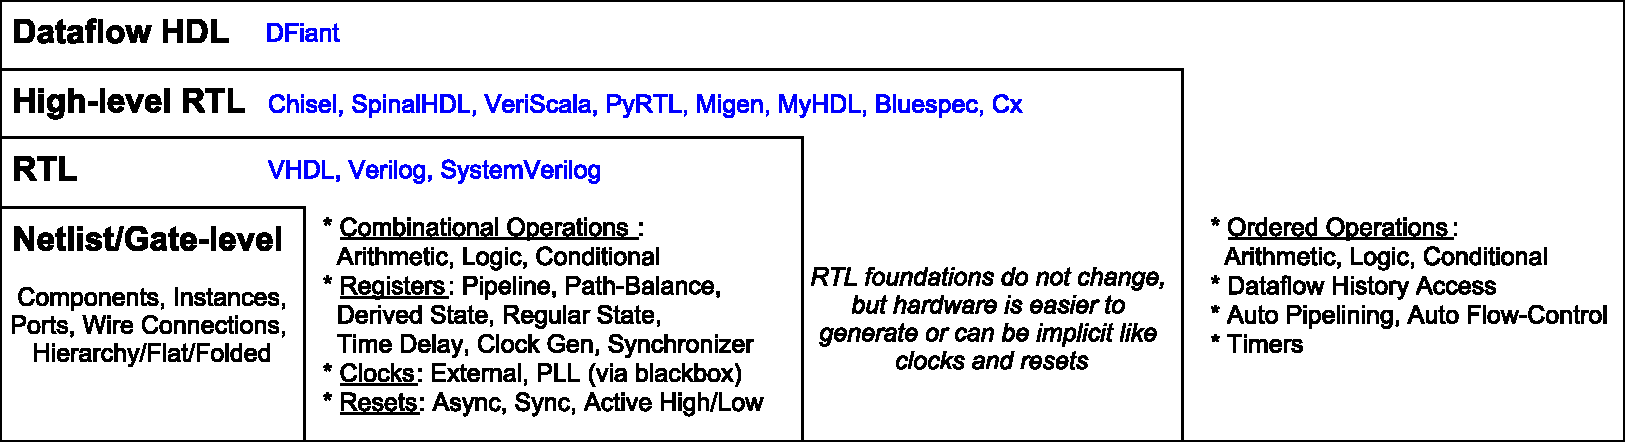
\includegraphics[width=\linewidth]{graphics/motivation.pdf} 
	\captionof{figure}{HDL abstraction layer summary (lowest=netlist, highest=dataflow) \\ DFiant is the first language to support the highest layer, a dataflow HDL.}
	\label{fig:motivation}
\end{figure*}

%\newpage %equivalent to when author names aren't removed
DFiant is implemented as a Scala library and relies on Scala's strong, extensible, and polymorphic type system to provide its own hardware-focused type system (e.g., bit-accurate dataflow types, input/output port types). The library performs two main tasks: the frontend compilation, which translates dataflow variable interactions into a dependency graph; and the backend compilation, which translates the graph into a pipelined RTL code and a TCL constraints file, followed by a hardware synthesis process using commercial tools. Additionally, the graph can be simulated within the Scala integrated development environment (IDE). 

This work focuses on the DFiant language and frontend compiler. DFiant is \emph{not} an RTL language, nor is it a sequential language such as C. The following two sections highlight DFiant's unique semantics by comparing them against modern design language alternatives. For a proof of concept, we implemented a preliminary auto-pipelining backend compiler to compare DFiant and traditional HDL design flows in two test cases: an Advanced Encryption Standard~\cite{pub2001197} (AES) cipher block and an IEEE-754~\cite{IEEE2008} floating point multiplier (FPMul). Future work may delve further into the backend compiler and its HLS potential.


The paper is organized as follows. The next section describes the motivation for the dataflow HDL abstraction layer, followed by Section~\ref{sec:dfiant}, which provides a general overview of the DFiant HDL language. 
Section~\ref{sec:evaluation} provides results, and finally, Section~\ref{sec:conclusion} concludes the paper.




%\newpage
%Interactions between DFiant types lead to hardware construction, while non-DFiant types (e.g. Integer) are considered as constants. 
 

%Modern designs are rich with arithmetic functionality. Surely the designer cannot explicitly pipeline everything manually and must be selective. On one hand, under-pipelining may lead to insufficient performance and redesign iterations. On the other hand, over-pipelining might lead to performance reduction due to limited room for logic and routing, in addition to wasting design time, energy, and device resources. 

%Typical FPGA devices now include clock generators, serializers, PCI express cores, internal memory blocks, external memory interfaces, and many other proprietary modules. Evidently, formulating designs that are transportable across devices and timing variance is difficult, if not impossible. Complex logic design has become a task fit only for experts. 
% The generic code annotations enabling this are cumbersome and limited. 




\section{A Dataflow Hardware Description Abstraction}
\label{sec:motivation}
In this section we detail how dataflow abstractions help decouple the functionality from its constraints. We also overview what dataflow HDL constructs are required to achieve maximum portable code. In the next section we demonstrate how these constructs are used in DFiant.

\fig{fig:motivation} summarizes the basic elements that make up HDLs at different abstraction layers, from a netlist up to the dataflow constructs presented in this paper. Each layer includes the expressive capabilities of the lowest layer (e.g., structural instance composition is possible in all HDLs). The layers are tagged with the relevant HDL names. Note that HLS languages and simulation constructs are not included in this summary. 

The basic notion of a dataflow abstraction is that instead of wires and registers we have dataflow token streams. This key difference between RTL and dataflow abstractions reveals why the former is coupled to device and timing constraints, while the latter is agnostic to them. Primarily, \emph{the RTL model requires designers to express what operations take place in each cycle, whereas the dataflow model only require the designer to order the operations based on their data dependencies}. More specifically, the RTL model utilizes combinational operations that must complete (their propagation delay) within a given cycle if fed to a register, while the dataflow abstraction only assumes order and not on which cycle operations begin or complete. By decoupling operations from fixed clock cycles the dataflow model enables the compilation toolchain to map operations to cycles and thereby independently pipeline the design. 

Furthermore, the RTL model requires designers to use registers for a variety of uses and thus binds the design to specific timing conditions. Specifically, we find three main uses for registers in the RTL model: \emph{synchronous technology backend}, \emph{synchronous technology interface}, and \emph{design functionality} (i.e., state). We now turn to discuss these different uses for registers and how the dataflow model can derive the first two uses without explicit user description.

\subsection{Synchronous Technology Backend Registers}
Registers are often required in a low-level design due to the underlying synchronous technology. Since they are unrelated to the functional requirement, a dataflow HDL can derive them automatically based on the functional requirements and design constraints. 
We differentiate between the following backend uses of registers:
\subsubsection{Pipelining and Path-Balancing}
Pipeline registers are inserted to split long combinational paths, and their placement is determined by designer-specified constraints, such as the maximum path cycle latency or the maximum propagation delay between registers. Pipelining increases the path cycle latency, and if the path converges with another path that requires no pipelining, then additional path-balancing registers are added to maintain correctness of the design. Because a balanced pipelining does not affect the design functionality, it can be automatically applied by the dataflow HDL compiler.   
\subsubsection{Synchronizers}
Clock domain crossing (CDC) and asynchronous signals are exposed to metastability. Synchronizers, often composed of registers, are used to mitigate its effect and bring the design to the proper reliability. Since we wish to have a clockless design frontend, we want the synchronizers to be implicit. A dataflow HDL compiler needs to infer synchronizers according to the design constraints without designer intervention. Note: our work currently focuses on single clock designs so the compiler we implemented does not yet support this feature.

\subsection{Synchronous Technology Interface Registers}
Functional design requirements are often accompanied by synchronous input/output (IO) timing constraints such as clocked protocol interfaces or real-time restrictions. However, these constraints only affect the interface and are unrelated to the design itself. To maximize design portability, we apply timed or legacy constructs \emph{solely in the periphery}, while coding the design core with only clockless dataflow constructs. We differentiate between the following synchronous signaling:
\subsubsection{External IO and Blackbox Interfaces}
External IOs that are exposed to the top design hierarchy or blackboxes that are exposed to the internal design core may impose synchronous protocols (e.g., data is valid one clock cycle after address is set). A dataflow HDL supports legacy RTL constructs to synchronously interface external IOs and instantiate blackboxes. 
\subsubsection{Timers}
Timers are design constructs for generating real-time signals or creating derivations of timed signal inputs. For example, a design using a 100MHz clock may drive a UART stream at 10Mbps or toggle a led at 1Hz. Rather than directly using registers as clock dividers or employing clock generation components (e.g., PLLs), one can create functional representation of their timed use-cases. A dataflow HDL has timer constructs that generate tokens at a given or derived rate. The compiler can take all clocks into consideration and generate the proper clock tree based on the available device resources and other design constraints. 

\subsection{Design Functionality (State) Registers}
Functional registers, or state, are needed when a design must access (previous) values that are no longer available on an input signal (e.g., cumulative sum or a state-machine's state). RTL designs invoke registers (behaviorally) to store the state. But, registers not only store the state, but also enforce specific cycle latencies. Furthermore, typical RTL languages declare additional variables and place extra assignments just to save the state. A dataflow HDL overcomes all these issues by including a construct to reuse a token from the stream history. Additionally, a related construct should set a token history to be used at initialization time.
We differentiate between two kinds of state: \textit{derived state}, and \textit{feedback state}. 


\subsubsection{Derived State} 
A derived state is a state whose current output value is \textit{independent} of its previous and can thereby be deduced by the compiler. For example, checking if a dataflow stream value has changed requires reusing the previous token and comparing to the current token. 

\subsubsection{Feedback State} 
A feedback state is a state whose current output value is \textit{dependent} on its previous state value. For example, the current cumulative sum value is dependent on the previous sum value. Therefore, a dataflow HDL requires not only to fetch previous token values, but also set the future state value. Addressable memory pools also hold feedback state (e.g., a processor register-file, memory blocks) and can be expressed as a large selectable state array or available dedicated memory components.

The two kinds of state differ heavily in performance improvement when the design is pipelined. A derived state path can produce a token for every clock tick, and pipelining a combination operation to reduce its cycle time will also increase its throughput. In contrast, a feedback state path is circular and cannot be pipelined as-is. 

Feedback state causes bottlenecks in many systems. For instance, a RISC-V processor program counter (PC) register manifests as a feedback state. The processor pipeline can only be improved thanks to a speculative mechanism that predicts the next PC value to prefetch instructions (e.g., PC+4 for a branch-not-taken prediction). In case of a miss-prediction other mechanisms take place. Further research may expand on dataflow abstractions that solve such problems functionally.

%\subsubsection{Speculated State} 
%A speculated state is a feedback state that can generate a new speculative value when the actual next value is unavailable.

%In some cases a feedback state limits the throughput too much. For example, a program counter (PC) register for a microprocessor pipeline. If we state dependent on the PC as a feedback state, it won't be possible for the pipeline to handle more than one instruction at a time. A known solution for this is to speculate on the next value of PC (good guess is branch not taken). If we guessed wrong the pipeline should ignore the prefetched instructions and restart from where the branch occurred. This allows us to generate new speculative tokens of PC, without waiting for the pipeline to supply the vi

%There is no actual dataflow feedback. 


\begin{table*}[t!]
  \centering
  \begin{minipage}[t][11.8cm][t]{0.505\linewidth}
    \centering
    \captionsetup{justification=centering}    
    \begin{minted}[xleftmargin=1em,linenos,autogobble,tabsize=2,framesep=1pt,frame=single,fontfamily=courier,fontsize=\fontsize{8}{9}\selectfont]{scala}
			import DFiant._
			
			trait MA4 extends DFDesign {
				val a    = DFSInt[16] <> IN init 0
				val b    = DFSInt[16] <> IN init 0
				val c    = DFSInt[16] <> IN init 0
				val d    = DFSInt[16] <> IN init 0
				val o    = DFSInt[16] <> OUT
				
				def ma(src : DFSInt[16]) = {     
					val acc = DFSInt[18] init 0    //-Compiled to->
					acc := acc - src.prev(4) + src //-Compiled to->
					(acc / 4).toWidth(16)
				}
				def avg2(src1 : DFSInt[16], src2 : DFSInt[16]) =
					((src1 + src2).wc / 2).toWidth(16)
					//  (_ + _).wc is a with-carry addition
					
				o := avg2(
					avg2(ma(a), ma(b)), avg2(ma(c), ma(d))
				)
			}
			
			
			
			
			
			
			
			
			
			object MA4App extends DFApp.VHDLCompiler[MA4]
    \end{minted}
    \captionof{figure}{The MA4 DFiant code \\ Concise and portable}
    \label{fig:MADFiant}
  \end{minipage}
  \hfill
  \begin{minipage}[t][11.8cm][t]{0.49\linewidth}
    \centering
    \captionsetup{justification=centering}
		\begin{minted}[xleftmargin=1em,autogobble,tabsize=2,framesep=1pt,frame=single,fontfamily=courier,fontsize=\fontsize{8}{9}\selectfont]{vhdl}
			...
			signal acc       : signed(17 downto 0);
			signal acc_prev1 : signed(17 downto 0);
			signal src_prev1 : signed(15 downto 0);
			signal src_prev2 : signed(15 downto 0);
			signal src_prev3 : signed(15 downto 0);
			signal src_prev4 : signed(15 downto 0);
			...
			sync_proc : process (CLK, RSTn)
			begin
			  if RSTn = '0' then
			    acc_prev1    <= 18d"0";
			    src_prev1    <= 16d"0";
			    src_prev2    <= 16d"0";
			    src_prev3    <= 16d"0";
			    src_prev4    <= 16d"0";
			  elsif rising_edge(CLK) then
			    acc_prev1    <= acc;
			    src_prev1    <= src;
			    src_prev2    <= src_prev1;
			    src_prev3    <= src_prev2;
			    src_prev4    <= src_prev3;
			  end if;
			end process sync_proc;
			...
			async_proc : process (all)
			  variable v_acc : signed(17 downto 0);
			begin
			  v_acc          := acc_prev1;
				v_acc 		     := v_acc - src_prev4 + src;
			  acc            <= v_acc;
			end process async_proc;
    \end{minted}
    \captionof{figure}{
    	The MA4 DFiant lines 11-12 compiled to VHDL \\ 
    	The DFiant code is extremely compact in comparison.
    }
    \label{fig:MAVHDL}
  \end{minipage}
%  \vfill
  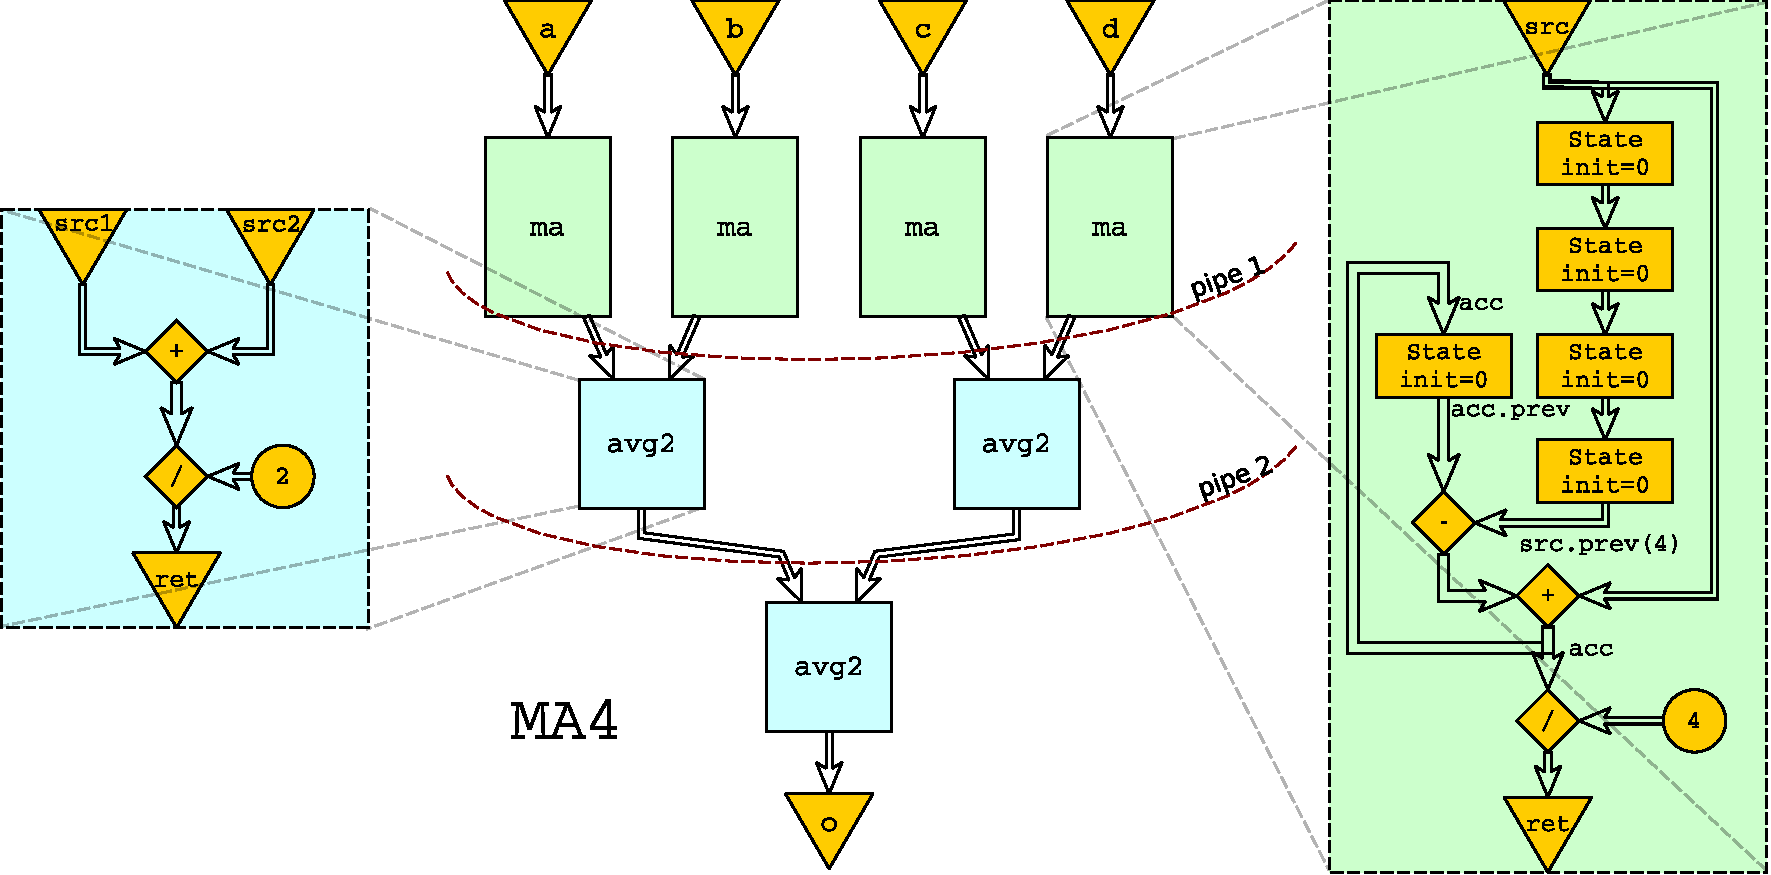
\includegraphics[width=0.92\linewidth]{graphics/ma.pdf}
  \captionsetup{justification=centering}
  \captionof{figure}{
  	The MA4 dataflow graph (the inputs are \code{a}, \code{b}, \code{c}, \code{d} and the output is \code{o}) \\ 
  	The entire design is a composition of the \code{ma} and \code{avg} functions (detailed blowouts are depicted as well). \\ 
  	The compiler places pipeline tags to achieve the required performance and the backend inserts registers accordingly. \\
  	The concurrent construction is implied from a sequential composition thanks to the dataflow abstraction. 
  }
\label{fig:MADraw}
\end{table*}

\section{The DFiant Language Overview}
\label{sec:dfiant}
DFiant is a Scala library and thus possesses various rich type safe language constructs. DFiant also incorporates unique language semantics that enable dataflow-based hardware description. Throughout this section we elaborate on these constructs and semantics via our running example, a four-by-four moving average (MA4) unit. The MA4 has four 16-bit integer input channels and is required to output the average of all channels, while each channel is averaged by a four-sample moving window continuously. The complete MA4 DFiant implementation and its equivalent dataflow graph are available in \fig{fig:MADFiant} and ~\ref{fig:MADraw}, respectively. \fig{fig:MAVHDL} presents a subset of the DFiant-generated VHDL (2008) code derived from lines 11-12 in \fig{fig:MADFiant}.


\subsection{Hello DFiant World!}
The DFiant code in \fig{fig:MADFiant} demonstrates the structure of any DFiant program: it imports the \code{DFiant} library (line 1), creates the top-level design by extending the \code{DFDesign} library abstract class (lines 3--21), and creates a runnable application that instantiates the top design trait, and compiles it into a VHDL file (line 32).

The MA4 design is fairly straightforward. Lines 4-8 generate the signed dataflow ports and include a \code{0} value initialization (see Section~\ref{sec:state_constructs}). 
Lines 10-14 define the function \code{ma} that generates a single four-sample moving average, while lines 15-16 define the function \code{avg2} that generates a two-input average unit. Finally, lines 18-20 compose \code{avg2} and \code{ma} to generate the entire MA4 functionality and assign it to the output port \code{o}. We elaborate on the unique DFiant constructs and semantics in the next sections.


\subsection{Dataflow Semantics}
DFiant code is expressed in a sequential manner yet employs an asynchronous dataflow programming model to enable an intuitive concurrent hardware description. For this purpose, DFiant applies the following rules:

\subsubsection{Concurrency and Execution Order} 
Concurrency is implicit and the data scheduling order, or \textit{token-flow}, is set by the \textit{data dependency}. DFiant schedules all independent dataflow expressions concurrently, while dependent operations are synthesized into a guarded FIFO-styled pipeline. The MA4 dataflow graph in \fig{fig:MADraw} demonstrates the concurrent paths constructed from the dataflow dependency. 

\subsubsection{Basic Operations} 
\label{sec:basic_ops}
Each application of an arithmetic/logic operator is translated into the appropriate hardware construction and applies a dataflow \emph{join} on their arguments. The arguments require a valid token for consumption to produce a new token generated from the operations. For example, \code{+} in \code{avg2} joins \code{src1} and \code{src2} and requires a token from both to produce the token \code{src1 + src2}.

\subsubsection{Path Divergence} 
\label{sec:path_div}
Diverging paths are implicitly \emph{forked}, so token production is possible if all target nodes are ready to consume the token. For example, \code{acc} result in \code{ma} is forked into a division operation and the state feedback.	It is impossible to consume an invalid token and once a token is consumed it is invalidated.

\subsubsection{Constants} 
Any Scala primitive value is considered as a constant when applied as an argument to a dataflow operation. For example, the value \code{2} in \code{avg2} is a primitive \code{Int} and is considered a constant in the division operation. Semantically, a constant is an infinite token generator that produces a new token with the same initial value each time the token is consumed.

\subsubsection{Pruning}
Unused nodes always consume tokens and are discarded during compilation. 


\subsection{State Constructs and Semantics}
\label{sec:state_constructs}
In contrary to RTL languages, DFiant does not directly expose register and wire constructs. Instead, DFiant assumes every dataflow variable is a stream and provides constructs to initialize the token history via the \code{.init} construct, reuse tokens via the \code{.prev} construct, and update the state via the \code{:=} construct. Lines 11-12 in \fig{fig:MADFiant} along with their compiled VHDL representation in \fig{fig:MAVHDL} demonstrate the state semantics as follows:

\subsubsection{Initialization} The \code{.init} construct is accompanied by one or more token values and only sets the initial state history. For example, line 11 constructs a dataflow variable and initializes all of its history as zero value tokens. The history sequence written from left to right sets tokens from newest to oldest, respectively. If the sequence is accessed beyond the oldest token than the oldest token is repeatedly produced. If the history is empty (not initialized) then stall bubble tokens are produced when accessed (see \sect{sec:stall_bubbles}). It is also possible to directly place bubble tokens in the history by writing either $\phi$ or \code{Bubble}.  

\subsubsection{History Access} The \code{.prev} construct reuses the previous state token. The very first "reused" token is the one set via \code{.init}. It is also possible to call \code{.prev(step)} with a step number argument to reuse older stream values. For any dataflow value \code{a} and a given positive integer \code{step}, a call to \code{a.prev(step)} is equivalent to repeated $step$ applications of \code{a.prev.prev...prev}.
For example, in line 12 we reuse a \code{src} token from four steps ago. If the \code{src} token stream is "$1,2,3,4,...$" with a $0$ initialization, then the \code{src.prev(4)} token stream is "$0,0,0,0,1,2,3,...$".

\subsubsection{Distributive Property} The history access via \code{.prev} is distributive over all the basic DFiant operations. For example, the distributed \code{a.prev + b.prev} is equivalent to \code{(a + b).prev}. 
 
\subsubsection{Stall Bubbles} 
\label{sec:stall_bubbles}
Invoking \code{.prev} on an uninitialized dataflow variable generates a stall bubble. Stall bubbles are consumed and produced like any other token, yet a basic operation with a stall bubble token must produce a stall bubble token. Additionally, stall bubbles do not affect a feedback state. The backend compiler is responsible to generate the additional logic required for existing design stalls. 

\subsubsection{State Update Scheduling} The new updated token is pushed into a dataflow stream by using the \code{:=} assignment construct. There can be more then one assignment to same variable, however only the last assignment updates the state and occurs when all dependent dataflow firing rules are satisfied. This rule is similar to signal update semantics in VHDL processes.

\subsubsection{Default Self-Generation} 
\label{sec:default_self_gen}
Any dataflow \code{a} variable has an implicit self-assignment \code{a := a.prev} that comes immediately after the variable construction. This creates an equivalent reference between \code{a} and \code{a.prev} which leads to a more intuitive programming.
For example, in line 12 we used \code{acc - ...} and not \code{acc.prev - ...}, since both expressions are equivalent.

\vspace{2ex}

Another example that illustrates the benefits of the DFiant state constructs is a 32-bit Fibonacci series generator implementation provided in \fig{fig:FibGen}. The dataflow version is shorter than its VHDL counterpart~\cite{fibgenvhdl} and greatly resembles the formal Fibonacci definition: $F_0 = 0$, $F_1 = 1$, $F_n = F_{n-1} + F_{n-2}$ for $n > 1$. 

\begin{figure}[h]
  \centering
  \captionsetup{justification=centering}    

  \begin{minted}[xleftmargin=0.15\linewidth, xrightmargin=0.15\linewidth,frame=single,autogobble,linenos,tabsize=2,fontfamily=courier,fontsize=\fontsize{8}{9}\selectfont]{scala}
    trait FibGen extends DFDesign {
      val o = DFUInt[32] <> OUT
      val f = DFUInt[32] init (1, 0)
      f := f.prev + f.prev(2)
      o := f.prev(2) //output from 0
    }
  \end{minted}
  \captionof{figure}{A DFiant 32-bit Fibonacci series generator \\ Great resemblance to the formal Fibonacci definition}
  \label{fig:FibGen}
\end{figure}

Both \fig{fig:MAVHDL} and \fig{fig:FibGen} emphasize the advantages of DFiant state constructs over RTL registers and wires.
One advantage is that the DFiant code resembles its RTL counterparts, but is also very concise since state elements are automatically constructed when a stream history is accessed. Another advantage is portability, because state elements are not registers and therefore any type of state component is applicable. Our first synchronous backend indeed maps state elements to registers, but even an asynchronous backend can compile the same code and apply the Muller C-element~\cite{muller1957theory} as a state element. 

\subsection{Conditional Constructs and Semantics}
DFiant has \code{ifdf} and \code{matchdf} conditional constructs which logically resemble the Scala \code{if} and \code{match}, respectively. These dataflow conditional constructs are also very similar to their RTL counterparts and yield multiplexer hardware. However, their semantics follow the same dataflow \emph{join} and \emph{fork} rules we described in Sections \ref{sec:basic_ops} and \ref{sec:path_div}, and therefore all dataflow values used within the conditional constructs are joined together and all modified dataflow variables which are referenced outside the conditional constructs are forked as well. Of course, the default compiler yields a simple combinational structure if there is no need for this additional flow control logic.

\fig{fig:SeqDet} demonstrates a simple DFiant finite state-match (FSM) design that detects the sequence "1001". The VHDL~\cite{seqdetvhdl} implementation is very similar but is mainly longer because the split between the sequential and combination parts is automatically done by the DFiant compiler.
Note we did not need to directly refer to \code{state.prev} at line 7, thanks to the default self generation described in \sect{sec:default_self_gen}.

\begin{figure}[t]
  \centering
  \captionsetup{justification=centering}    
  
  \begin{minted}[xleftmargin=0.08\linewidth, xrightmargin=0.08\linewidth,frame=single,autogobble,linenos,tabsize=2,fontfamily=courier,fontsize=\fontsize{8}{9}\selectfont]{scala}
    trait SeqDet extends DFDesign {
      val seqIn  = DFBool() <> IN
      val detOut = DFBool() <> OUT
      object State extends Enum.Auto {
        val S0, S1, S10, S100, S1001 = Entry
      }
      val state = DFEnum(State) init State.S0
      matchdf(state)
      .casedf(State.S0) {
        detOut := 0
        ifdf (seqIn) {state := State.S1}
        .elsedf      {state := State.S0}
      }.casedf(State.S1) {
        detOut := 0
        ifdf (seqIn) {state := State.S1}
        .elsedf      {state := State.S10}
      }.casedf(State.S10) {
        detOut := 0
        ifdf (seqIn) {state := State.S1}
        .elsedf      {state := State.S100}
      }.casedf(State.S100) {
        detOut := 0
        ifdf (seqIn) {state := State.S1001}
        .elsedf      {state := State.S0}
      }.casedf(State.S1001) {
        detOut := 1
        ifdf (seqIn) {state := State.S1}
        .elsedf      {state := State.S10}
      }
    }
  \end{minted}
  \captionof{figure}{A DFiant "1001" sequence detector FSM \\ Very similar to its VHDL counterpart}
  \label{fig:SeqDet}
\end{figure}


%\subsection{Mutability}
%\label{sec:mutability}
%`:=` used to set update the state.
%DFiant supports dataflow variables mutability via the \code{:=} operator. Do not confuse with Scala-level mutability which is enabled by using \code{var} instead of \code{val}. Each dataflow class has two variations: an immutable class, which inherits from \code{DFAny\textbf{Val}} and a mutable class, which inherits from \code{DFAny\textbf{Var}} and accepts \code{:=}. The difference between the types enforces an immutable right-hand-side (RHS), where required, and a mutable variable creation. Consider, for instance, the DFiant implementation of \code{g} in Table \ref{tbl:StateExDefImpl}: \code{a} is immutable because it is a RHS addition between the dataflow variable \code{i} and a literal value \code{5}. Contrarily, \code{c} is mutable, since it is a dataflow variable constructor (\code{.init} constructs a new initialized variable, while preserving the mutability trait). 
%
%Fig.~\ref{fig:Inherit} demonstrates a dual class definition for every type  (immutable and mutable). The naming convention helps to reason about the mutability. For example, \code{DFBits} and \code{DFBits.Var} are immutable and mutable classes, respectively. Constructing a new variable via \code{DFBits} (e.g, \code{val a = DFBits[5]}) returns the mutable \code{DFBits.Var[5]}. Usually, we either receive or return an immutable type, hence we do not require annotating a type with its mutable variation. In cases where we want to return a mutable type, we annotate it as an output port (see Section~\ref{sec:io_ports}).
%
%DFiant's code safety is enforced by maintaining the 'DF-mutability' trait while aliasing (accepting the ':=' operator). This means that an alias of a \textbf{Var}, is still a \textbf{Var}, and can be assigned, while an alias of a \textbf{Val} cannot. This concept is illustrated in ???, and further explained in ???:


\subsection{Hierarchy and Connectivity}
So far, all examples demonstrated a single dataflow design without any hierarchies. The MA4 design managed to create structural encapsulations and composition via Scala definitions. Earlier, in \sect{sec:motivation}, we stressed the importance of any HDL to support hierarchies via constructs that describe components, ports and their connections. For this purpose DFiant utilizes the symbols \code{<>} to both construct dataflow ports and create connections between them.
when applied between a dataflow variable constructor 

\begin{table*}[t!]
  \small
  \begin{minipage}[t][9cm][t]{0.343\linewidth}
    \centering
    \captionsetup{justification=centering}
    \begin{minted}[xleftmargin=1em,linenos,autogobble,tabsize=2,framesep=1pt,frame=single,fontfamily=courier,fontsize=\fontsize{7}{8}\selectfont]{scala}
      //All networks have the same interface
      trait Network extends DFDesign {
        val iT = DFSInt[16] <> IN  //Top
        val iB = DFSInt[16] <> IN  //Bottom
        val oT = DFSInt[16] <> OUT //Top
        val oB = DFSInt[16] <> OUT //Bottom
      }
      //State in Top Connection
      trait NWLeft extends Network {
        iT.prev <> oT //Connection
        oB := iB + 5  //Assignment
      }
      //State in Bottom Assignment
      trait NWRight extends Network {
        iT <> oT * 3  //Connection
        oB := iB.prev //Assignment
      }
      //Parent box includes two sibling boxes
      trait NWParent extends Network {
        iT init (5, 7) //Initializing history
        iB init (2, 6) //Initializing history
        val nwL = new NWLeft {}
        val nwL = new NWRight {}
        nwL.iT <> iT
        nwL.iB <> iB
        nwR.oT <> oT
        nwR.oB <> oB
      }
      //Direct connections between siblings
      trait NWParDirect extends NWParent {
        nwL.oT <> nwR.iT
        nwL.oB <> nwR.iB
      }
      //Cross connections between siblings
      trait NWParCross extends NWParent {
        nwL.oT <> nwR.iB
        nwL.oB <> nwR.iT
      }
    \end{minted}
    \vfill
    \captionof{figure}{Various network designs \\ Featuring hierarchies and inheritance }
    \label{fig:BoxTopCode}
  \end{minipage}%
  \hfill
  \begin{minipage}[t][12cm][b]{0.64\linewidth}
    \centering
    \captionsetup{justification=centering}
    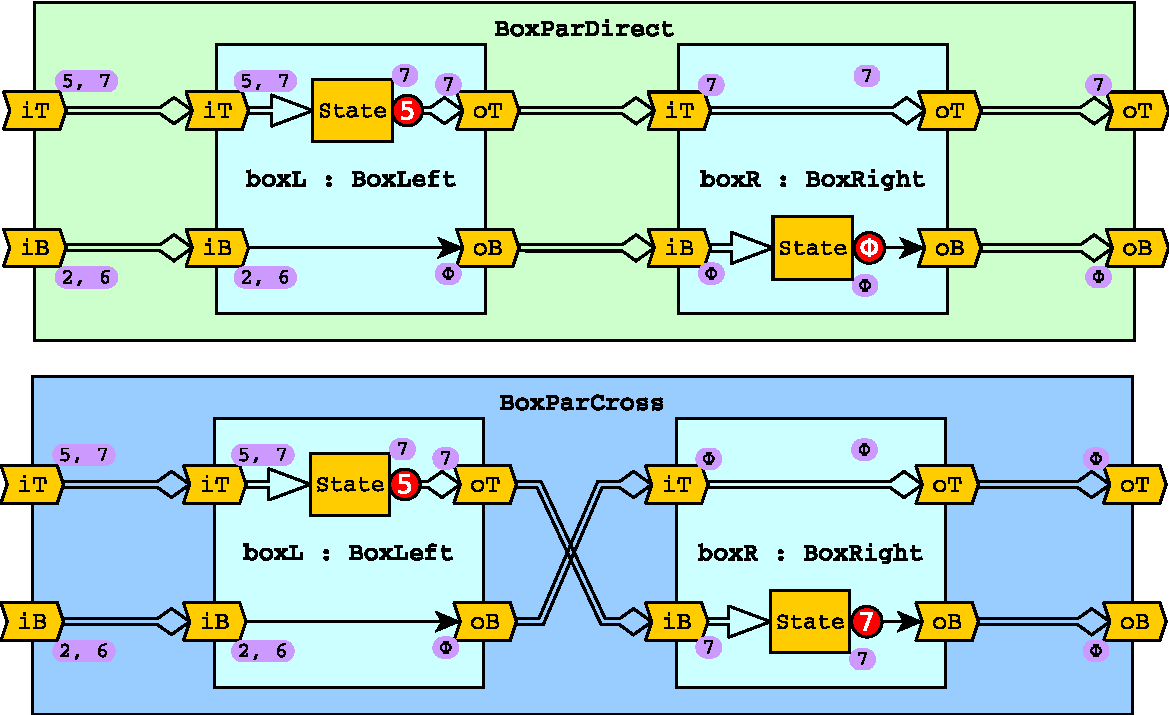
\includegraphics[width=0.9\linewidth]{graphics/connectivity.pdf}
    \captionof{figure}{
      Hierarichal drawing of \code{NWParDirect} and \code{NWParCross} \\
      The \colorbox{initcolor}{purple} numbers mark the initialization history as it is propagated according to the semantic rules of DFiant. The \colorbox{red}{\textcolor{white}{red}} numbers mark initial tokens generated by the state elements.
    }
    \vfill
    \label{fig:BoxTopDraw}
    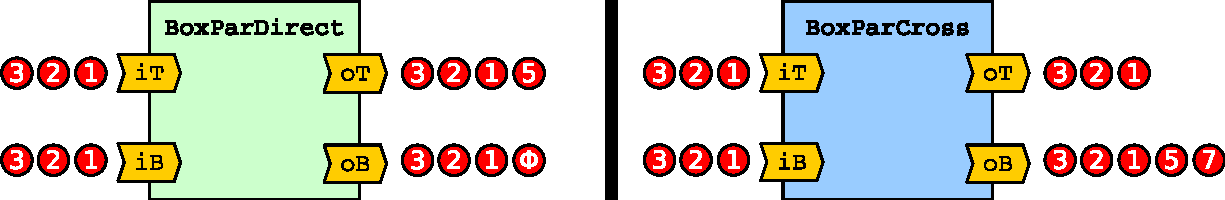
\includegraphics[width=0.9\linewidth]{graphics/connectivityTokens.pdf}
    \captionof{figure}{
      Input/Output token flow example to/from the two parent boxes (the rightmost tokens are the oldest). 
    }
    \label{fig:BoxTopTokens}
  \end{minipage}%
  \vspace{2ex}
  \hrule
  \vspace{2ex}
  \captionof{table}{Connection \code{<>} and Assignment \code{:=} Operator Comparison}
  \label{tbl:Box}
  \begin{tabular}{|c|c|c|}
    \hline 
    \textbf{Criteria} & \textbf{Connection \code{<>}} & \textbf{Assignment \code{:=}} \\ 
    \hline
    \begin{minipage}{0.1\textwidth}
      \flushleft
      Code
    \end{minipage} 
    &
    \begin{minipage}[c][1.5cm]{0.4\textwidth}
      \begin{minted}[autogobble,tabsize=2,framesep=1pt,fontfamily=pcr,fontsize=\fontsize{7}{8}\selectfont]{scala}
      trait IOConnection extends DFDesign {
        val i = DFUInt[8] <> IN
        val o = DFUInt[8] <> OUT
        o <> i
      }
      \end{minted}
    \end{minipage} 
    &  
    \begin{minipage}[c][1.5cm]{0.4\textwidth}
      \begin{minted}[autogobble,tabsize=2,framesep=1pt,fontfamily=pcr,fontsize=\fontsize{7}{8}\selectfont]{scala}
        trait IOAssignment extends DFDesign {
          val i = DFUInt[8] <> IN
          val o = DFUInt[8] <> OUT
          o := i
        }
      \end{minted}
    \end{minipage} 
    \\ 
    \hline 
    \begin{minipage}{0.1\textwidth}
      \flushleft
      Functional Diagram
    \end{minipage} 
    &
    \begin{minipage}[c][2cm]{0.10\textwidth}
      \centering
      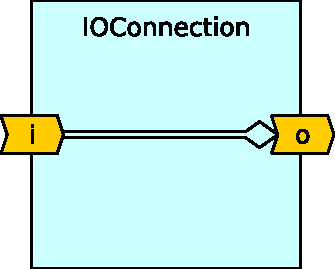
\includegraphics[height=1.8cm]{graphics/IOConnection.pdf}\\
    \end{minipage}%
    \hfill 
    \begin{minipage}[c][2cm]{0.27\textwidth}
      A double line arrow indicates a dataflow dependency \textbf{with} an initial condition dependency.
    \end{minipage} 
    &  
    \begin{minipage}[c][2cm]{0.10\textwidth}
      \centering
      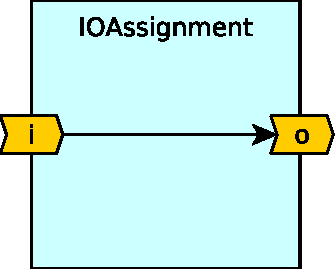
\includegraphics[height=1.8cm]{graphics/IOAssignment.pdf}\\
    \end{minipage}%
    \hfill 
    \begin{minipage}[c][2cm]{0.27\textwidth}
      A single line arrow indicates a dataflow dependency \textbf{without} affecting initial conditions of the consumer.
    \end{minipage} 
    \\ 
    \hline
    \begin{minipage}{0.1\textwidth}
      \flushleft
      Directionality \\and\\ Commutativity
    \end{minipage} 
    &
    \begin{minipage}[c][1.5cm]{0.42\textwidth}
      The operator is commutative, meaning \code{a <> b} is equivalent to \code{b <> a}. One argument is the \emph{producer}, while the other is the \emph{consumer}. The dataflow direction is sensitive to the context in which the operator is applied.
    \end{minipage} 
    &  
    \begin{minipage}[c][1.5cm]{0.42\textwidth}
      The operator is non-commutative, meaning \code{a := b} determines that \code{b} is the \emph{producer}, transferring data to the \emph{consumer} \code{a}.
    \end{minipage} 
    \\ 
    \hline
    \begin{minipage}{0.1\textwidth}
      Initialization
    \end{minipage} 
    &
    \begin{minipage}[c][1.2cm]{0.42\textwidth}
      Initialization is transferred to the consumer. If the consumer has both initialization via \code{.init} and connection, then the \code{.init} is the one that takes effect.
    \end{minipage} 
    &  
    \begin{minipage}[c][1.2cm]{0.42\textwidth}
      The consumer initialization is \textbf{not} affected.
    \end{minipage} 
    \\ 
    \hline
    \begin{minipage}{0.1\textwidth}
      \flushleft
      Mutation
    \end{minipage} 
    &
    \begin{minipage}[c][0.5cm]{0.42\textwidth}
      A consumer can only be connected once at each bit.
    \end{minipage} 
    &  
    \begin{minipage}[c][0.5cm]{0.42\textwidth}
      The same bit in a consumer can be assigned to 
    \end{minipage} 
    \\ 
    \hline
    \begin{minipage}{0.1\textwidth}
      \flushleft
      Statement Order
    \end{minipage} 
    &
    \begin{minipage}[c][0.8cm]{0.42\textwidth}
      Connections statements can be placed in any order. Connection from assigned variable TBD 
    \end{minipage} 
    &  
    \begin{minipage}[c][0.8cm]{0.42\textwidth}
      TBD.
    \end{minipage}% 
    \\ 
    \hline
  \end{tabular}% 
\end{table*}


%\subsection{IO Ports}
%\label{sec:io_ports}
%The class \textit{Box} from Table~\ref{tbl:Box} can also be coded as demonstrated in Fig.~\ref{fig:IOBox}. The annotation \code{DFVar $<>$ Dir} controls \textit{DFVar}'s access by encapsulating the variable with the dataflow port class, \code{DFPort}: an \code{IN} port can only be read (immutable), while an \code{OUT} port can only be modified (unreadable). DFiant has implicit conversions in place that selectively converts between \code{DFPort} and \code{DFAny} instances, without breaking mutability rules and type safety. The port annotations match the capabilities of traditional HDLs, and are noticeably absent from HLS languages such as C++. 

\subsection{Structural Composition and Generation}
DFiant expands traditional structural composition capabilities by utilizing Scala's object oriented features such as inheritance and polymorphism, as well as finite loops and recursive composition. The hierarchical compositions provide the scope and dependencies for the dataflow variables. The hierarchy itself is transparent to the dataflow graph, as if the entire design is flattened, inlined, and unrolled. Therefore, hierarchies in DFiant are synthesizable, highly reusable, and do not affect the design performance (may affect compilation time). 


\subsection{Bit-Accurate Operations and Type Inference}
DFiant supports various basic dataflow types such as \code{DFBool}, \code{DFBits}, \code{DFUInt}, and \code{DFSInt}.
All DFiant's dataflow types are bit-accurate and structurally static, with their bit-width set upon construction (e.g., \code{DFBits[5]} is a 5-bit vector). Operations between dataflow variables produce a bit-accurate result with the proper type inference. For example, an addition between an unsigned 5-bit variable (\code{DFUInt[5]}) and a signed 10-bit variable (\code{DFSInt[10]}) produces an adder that can be implicitly converted to a 10-bit signed variable, if carry is not required, or an 11-bit signed variable by explicitly invoking \code{.wc} from the addition. DFiant also allows operations between dataflow types and their corresponding Scala numeric types, by treating the Scala numeric types as constants (e.g., addition between \code{DFSInt} and \code{Int} variables). 


\subsection{Bit Aliasing and Casting}
Aliasing in DFiant enables referencing a part of a dataflow variable, by invoking \code{.bits(hiIdx, loIdx)}, which creates a bits vector alias that references the original variable at the given index parameters. Every change of a dataflow variable affects its alias and vice versa (similar to VHDL's signal aliasing). Since this function also casts the variable as \code{DFBits}, this feature is used as a raw-data cast between different dataflow types. Aliasing of an alias is also possible, while maintaining relative bits indexing. Aliasing preserves the mutability trait: an alias of an immutable variable is immutable, while an alias of a mutable variable is mutable. 


Fig.~\ref{fig:Aliasing} demonstrates aliasing code and its effect on the contents of a dataflow variable (\code{bits128}). Each line code does as follows:
\begin{enumerate}
  \item Constructs a new 128-bit vector, \code{bits128}, and clears it.
  \item Creates a new alias, \code{alias64}, which references the most significant 64 bits of \code{bits128}. Since \code{bits128} is a \code{DFBits} variable, there is no need to invoke \code{.bits()}, and we can apply the required indexes directly.
  \item Creates a new alias, \code{alias32}, which references the least significant 32 bits of \code{alias64}, which reference bits 64 to 95 of \code{bits128}.
  \item Constructs a new double precision floating point dataflow variable, \code{dbl}, and initialize its value as \code{1.0} (hexadecimal value of \code{0x3FF00...0}).
  \item Modifies the least significant byte of \code{dbl}.
  \item Sets the most significant bit of \code{bits128}.
  \item Assigns \code{dbl} to the least significant 64 bits of \code{bits128} through casting. All the bits of \code{dbl} are selected because \code{.bits()} is invoked without index parameters.
  \item Modifies a byte of \code{bits128}.
  
\end{enumerate}

\begin{figure}[h]
  \centering
  \begin{minipage}[b][3cm][b]{0.57\linewidth}
    \vfill
    \begin{minted}[xleftmargin=1.5em,linenos,autogobble,tabsize=2,framesep=1pt, frame=single,fontsize=\fontsize{8}{8}\selectfont]{scala}
      val bits128 = DFBits[128] := 0
      val alias64 = bits128(127, 64)
      val alias32 = alias64(31, 0)
      val dbl = DFDouble() := 1.0
      dbl.bits(7,0) := 0x28
      bits128(127) := 1
      bits128(63, 0) := dbl.bits()
      alias32(16, 8) := 0x57		    
    \end{minted}
    \vfill
    \subcaption{DFiant code}
  \end{minipage}%
  \hfill
  \begin{minipage}[b][3cm][b]{0.42\linewidth}
    \centering
    \vfill
		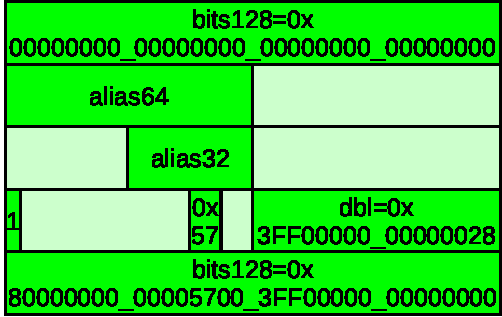
\includegraphics[width=\linewidth]{graphics/Aliasing.pdf} 
    \vfill
    \subcaption{Contents of \code{bits128}}
  \end{minipage}
  \captionof{figure}{Bit aliasing and casting example}
  \label{fig:Aliasing}
\end{figure}


\subsection{Simulation Constructs}
\label{sec:simulation}
Unlike VHDL and Verilog which were developed for simulation and only later were adapted for synthesis, DFiant was developed with focus on being a synthesizable language. Nonetheless, to test our designs we added some basic simulation-only constructs. To clearly separate pure simulation constructs from the rest of the language, we placed them under a separate name space -- \code{sim}. Additionally, all simulation constructs exist only within a simulation context. A simulation context is formed within a derivative of a dataflow design called \code{DFSimulation}. The \code{DFSimulation} construct is typically a toplevel instance that holds both our device-under-test (DUT) and the testing logic. Currently, the DFiant compiler only supports a handful of dedicated simulation constructs:
\code{sim.assert} to print errors if a condition is not satisfied; \code{sim.report} for printing messages; and finally \code{sim.finish} to finish the simulation. 
%All these constructs are very similar to their VHDL counterparts and in fact are



%+ C has no clear input/output notation. Input array and output array are the same.
%
%+ IDE: Intellisense, error highlighting, code completion, watches, println.
%+ Unified compilation
%+ Complete project build with the IDE. Compile results.
%Yes abstract away pipelining. No to scheduling control.
%
%Features we don't want
%simulations constructs.
%separate constraints file.
%
%VHDL Possible race conditions.
%
%
%+Include a summary table of RTL feature abstraction and how their are defined in DFiant.


\section{The DFiant Compiler}
\label{sec:compiler}
TBD

\subsection{Frontend Compiler}
%The DFiant frontend compiler relies mostly on the Scala compiler since DFiant is embedded as Scala library, and therefore has strong type-safe protection. DFiant is an early-adopter of new Scala features such as literal types~\cite{TypeLevelScala} and operations~\cite{singleton-ops}, which further improve type safety (e.g., a \code{DFBits[5].bits(Hi,Lo)} bit selection is compile-time-constrained within the 5-bits vector width confines). 

\subsection{Backend Compiler}
\subsubsection{Automatic Pipelining, Path-Balancing and Flow-Control}

The dataflow abstraction enables designers to describe hardware without explicitly pipelining the design. The DFiant backend compiler automatically pipelines the design and places registers to split long combinational paths. The compiler works with a propagation delay (PD) estimation database that can be tailored for any target device and technology. With this information and a target clock constraint the compiler tags the dataflow graph with the additional pipe stages required before producing the RTL code. One possible tagging is depicted in \fig{fig:MADraw}, in which two pipe stages were added between the large operations. Depending on the availability of DSP blocks in the target device, it is also possible to break the basic operations to multiple cycles by instantiating the proper vendor IP (e.g., a long multiplication operation should require several cycles). All of these target-specific adaptations are done without designer intervention and thus make any DFiant design highly portable.

To maintain design correctness the compiler adds path-balancing registers when pipeline registers are added and different-latency paths converge. Since these two features are separate, we can allow designers to explicitly place pipe stages in critical junctions should our PD estimation fail. The \code{.pipe} construct adds a pipe stage at a specific node and the compiler will balance the rest of the converging paths. While both \code{.pipe} and \code{.prev} constructs appear similar, the \code{.prev} construct does affect the path-balancing mechanism. For example, \code{x - x.prev} create a derivation circuit while \code{x - x.pipe} will result in a constant zero since path-balancing applied at the subtraction input arguments results in a \code{x.pipe - x.pipe} operation.

The asynchronous nature of DFiant means the compiler can adapt the design to any FIFO ready-valid signaling for automatic flow-control. For example, the MA4 RTL interface can have ready-valid signaling to each of its input and output ports to allow backpressure. To achieve this manually in RTL is extremely error-prone, while the DFiant generated RTL code stays true to the original dataflow description, and therefore, correct.
 
In \sect{sec:motivation} we discussed the problem when attempting to pipeline a feedback state. The \code{ma} function creates the feedback state referenced via the \code{acc} variable. The \code{ma} blowout in \fig{fig:MADraw} exposes this problem by having a circular feedback that updates the \code{acc} state. This feedback cannot be pipelined as-is because path-balancing will never be able to satisfy the balancing rule due to circular path dependency. It is only possible to increase the clock rate in feedback circuitry by applying multi-cycle or speculative logic (e.g., a RISC-V processor core contains several feedback junctions like the PC update and therefore has single-clock, multi-cycle and speculation-based pipelined implementations). 

\subsubsection{Resource Optimizations} 
TBD
%Resource optimizations can be target agnostic or target specific.
%We experimented with a handful of target agnostic optimization techniques: pruning of unconnected pathways and variants of constant propagation. The greatest potential for optimization is re


\subsubsection{Legible RTL Generation} TBD

\subsubsection{Simulation Generation} TBD

\section{Results}
\label{sec:evaluation}
In this section we present a working proof of concept by implementing two case studies: an AES cypher, and a double precision FPMul. We compare both test cases against traditional designs, and demonstrate competing performance while simplifying code verbosity significantly. 

%{Brainstorming}
Explicitly saving history for sample
Thanks to type inference, no need to declare types for internal values.
No need to extend the a value to get a carried result.
No need to create explicit pipeline (which also changed according to the target device).
No need to explicitly create stall logic.
We are replacing concepts of register and wire to state and stateless. This is key difference between dataflow 
and RTL HDLs. Dataflow assumes there is always a history, in every dataflow value. So we can access the history, yet call it stateless.


%\subsection{Methodology}
%We implemented both test cases in DFiant, constrained them by a variance of minimum frequency requirements, and compiled them to RTL. The DFiant compiler automatically pipelined the design to achieve the required minimum frequency, and generated an RTL verilog file and a TCL constraints file. For a baseline we obtained equivalent open-source RTL cores and Vivado HLS implementations, where possible. We disabled the DFiant backend support for pipelined valid/ready signaling and a blocking back-pressure, since the RTL cores did not support this capability.
%
%We chose the following comparison metrics: the maximum clock frequency, clock cycle latency, utilizations of both look-up tables (LUTs) and flip-flop registers (FFs), and lines of code (LoC). Digital signal processing (DSP) block utilization was zero for AES and equivalent for FPMul across all designs, thus neglected from the table. We used Xilinx Vivado to synthesize and implement the RTL design for a Virtex-7 FPGA, part number: xc7vx485tffg1761-2. The tool was configured to use default strategy for both synthesis and implementation processes. For each design, we recorded the maximum clock frequency, LUTs, and FFs. We recorded the design latency as reported by the DFiant and Vivado HLS compilers, and the RTL cores documentation. Finally, we automatically counted the LoC \cite{danial2009cloc}, applied standard score normalization (0-100) to all metrics, and assured higher values indicate better score for all metrics. Mean score of all metrics is presented as well.
%
%\subsection{Case Study: AES Cypher}
%For baseline comparison we used three AES cypher RTL designs from opencores.org: Das core \cite{das2010fully}, Hsing core \cite{hsing2013aes} and Salah core \cite{salah2013aespipe}. Additionally, we obtained a Vivado C++ HLS design~\cite{oflynn2014rapid}. All these designs are fully pipelined, meaning that in every cycle the design accepts new key and data inputs, and emits an encrypted data output, delayed by a fixed design latency.
%
%We compiled the DFiant and Vivado HLS designs with three target clock frequencies: 200 MHz, 300 MHz, and 450 MHz. We named the designs accordingly (e.g., DFiant\_200 is the 200MHz target design). We collected the results in Table~\ref{tbl:AES_Compare_Table}, and displayed their normalized standard score in Fig.~\ref{fig:AES_Compare_Graph}. We added the supported key types quantity as a metric, since some designs support 128bit keys and do not include 192bit and 256bit keys as well. The table also includes an 'SBox BRAM Use' column, since some designs do not use memory to implement the AES SBox function.
%
%%\begin{table*}[t!]
%%  \centering
%%  \begin{minipage}[t][5cm][t]{0.62\linewidth}
%%    \centering
%%    \captionof{table}{AES Cypher RTL Designs Comparison\\(the numbering on the left associates configurations with \fig{fig:AES_Compare_Graph})}
%%    \label{tbl:AES_Compare_Table}
%%    \includegraphics[scale=1]{graphics/AES_Compare_Table.pdf} 
%%  \end{minipage}
%%  \hfill
%%  \begin{minipage}[t][5cm][t]{0.37\linewidth}
%%    \centering
%%    \captionof{table}{FP Mult. RTL Designs Comparison\\(the numbering on the left associates configurations with \fig{fig:FP_Compare_Graph})}
%%    \label{tbl:FP_Compare_Table}
%%    \includegraphics[scale=1]{graphics/FP_Compare_Table.pdf} 
%%  \end{minipage}
%%  \begin{minipage}[b][3.8cm][b]{0.62\linewidth}
%%  	\centering
%%    \includegraphics[height=3cm]{graphics/AES_Compare.pdf} 
%%    \captionof{figure}{AES cypher RTL designs score comparison (higher = better)\\ \quad}
%%    \label{fig:AES_Compare_Graph}
%%  \end{minipage}
%%  \hfill
%%  \begin{minipage}[b][3.8cm][b]{0.37\linewidth}
%%    \centering
%%    \includegraphics[height=3cm]{graphics/FP_Compare.pdf} 
%%    \captionof{figure}{FP multiplication RTL designs score comparison (higher = better)}
%%    \label{fig:FP_Compare_Graph}
%%  \end{minipage}
%%\end{table*}
%
%The Hsing core clearly has the best performance among the different designs (but the lowest score on LUTs utilization). The primary reason it achieved this is because it uses LUTs instead of BRAMs. This enables the synthesizer to optimize the AES SBox function, and even pipeline it. DFiant uses its \code{lookupTable} library function to implement SBox, and we have yet to enable such an option for DFiant. 
%
%Although the DFiant-generated RTL performance is not optimal, it can still  be improved without modifying the DFiant AES code, if the DFiant compiler is optimized. Moreover, this code has an adaptive pipeline, while the RTL cores pipelines are fixed. The Vivado implementation enjoys the same advantages as DFiant, and has even less LoC. However, the Vivado code does not support all possible keys and its maximum performance is far from optimum (we did not attempt to improve the HLS pragma directives).
%
%If we assume all metrics have the same weight, the mean score places the DFiant solutions at the top. It is difficult to determine what is truly the best solution, but DFiant clearly has the best potential for further improvement without any modification to the application code.
%
%           
%\subsection{Case Study: Double Precision FPMul}
%
%We compared our FPMul with the open IEEE-754 compatible Lundgren core \cite{lundgren2014open} (the only IEEE-754 fully compatible FPMul RTL design we had access to). Since the core is a complete floating point unit, we disabled the unnecessary parts, reducing it to only an FPMul, for a fair comparison with DFiant's code. The DFiant code was written by using the Lundgren VHDL code as a reference design. The designs are very similar in their structure, except that DFiant is considerably less verbose, and has no explicit pipeline.
%
%We had no access to an open Vivado HLS FPMul for comparison. We could have directly invoked a \code{double} multiplication, but an inspection of the generated RTL revealed that Vivado HLS just instantiates an RTL floating point blackbox core. DFiant can choose to use this core as well, and achieve identical performance to Vivado HLS. Furthermore, the Vivado HLS floating point implementation is not fully compatible with IEEE-754 (e.g, does not support denormalized numbers).
%
%Similarly to the AES case study, we collected the results in Table~\ref{tbl:FP_Compare_Table}, and displayed their normalized standard score in Fig.~\ref{fig:FP_Compare_Graph}. In comparison with the Lundgren core, DFiant\_350 is better in every criteria, aside from FFs utilization. Ultimately, DFiant out-performs its reference design of FPMul, and demonstrates its ability to provide different RTL designs for design space exploration.


\section{Conclusion}
\label{sec:conclusion}
In this paper we proposed a novel DF-HDL abstraction layer that goes beyond RTL to free designs from being coupled to specific device or timing constraints. This abstraction layer tosses aside the register and wire RTL foundation blocks in favor of dataflow principles discussed in \sect{sec:motivation}. We also evolved the DFiant HDL and compiler to support dataflow state and many other useful constructs. DFiant provides a seamless concurrent programming approach, and yet it still facilitates a versatile compositional and hierarchical expressiveness. 

To evaluate the DFiant language and compiler, we reimplemented various RTL designs in DFiant and compared their performance, utilization, and LoCs. We demonstrated that most DFiant designs have equivalent performance and utilization to their RTL counterparts, yet manage to save between 50\% to 70\% LoCs. Evidently, the potential to increase designer productivity is significant, but notwithstanding, the greatest potential of DFiant is laid not in its concise syntax, but in its agnostic hardware description.  


Future work may explore dedicated simulation backend, an asynchronous logic backend, support for dynamic dataflow, or the missing abstractions like \emph{timers} (see \sect{sec:sync}).

%%%%%%%%%%%%%%%%%%%%%%%%%%%%%%%%%%%%%%%%%%%%%%%%%%%%%%%%%%%%%%%%%%%%%%%%%%%%%%%%%%


%%%%%%%%%%%%%%%%%%%%%%%%%%%%%%%%%%%%%%%%%%%%%%%%%%%%%%%%%%%%%%%%%%%%%%%%%%%%%%%%%%
% Acknowledgement
%%%%%%%%%%%%%%%%%%%%%%%%%%%%%%%%%%%%%%%%%%%%%%%%%%%%%%%%%%%%%%%%%%%%%%%%%%%%%%%%%%
%%
%% The acknowledgments section is defined using the "acks" environment
%% (and NOT an unnumbered section). This ensures the proper
%% identification of the section in the article metadata, and the
%% consistent spelling of the heading.
%\begin{acks}
%LEGaTO ack here
%\end{acks}
%%%%%%%%%%%%%%%%%%%%%%%%%%%%%%%%%%%%%%%%%%%%%%%%%%%%%%%%%%%%%%%%%%%%%%%%%%%%%%%%%%


%%%%%%%%%%%%%%%%%%%%%%%%%%%%%%%%%%%%%%%%%%%%%%%%%%%%%%%%%%%%%%%%%%%%%%%%%%%%%%%%%%
% Bibliography
%%%%%%%%%%%%%%%%%%%%%%%%%%%%%%%%%%%%%%%%%%%%%%%%%%%%%%%%%%%%%%%%%%%%%%%%%%%%%%%%%%
%%
%% The next two lines define the bibliography style to be used, and
%% the bibliography file.
\bibliographystyle{ACM-Reference-Format}
\bibliography{bib/macros,bib/references}
%%%%%%%%%%%%%%%%%%%%%%%%%%%%%%%%%%%%%%%%%%%%%%%%%%%%%%%%%%%%%%%%%%%%%%%%%%%%%%%%%%



\end{document}
\endinput